\chapter{地下探测FDTD仿真技术研究}
本章的主要是内容是探地雷达应用到地下目标探测时的仿真技术。在将深度学习相关技术,特别是深度卷积神经网络
技术应用到探地雷达地下目标识别时需要提供大量的训练与测试数据用于神经网络的性能调优、结构调整、参数选择等等
过程。由于电磁仿真所得的数据具有目标位置明确模型参数已知的特点,在进行神经网络建模时就有了明确的参考
依据,可以验证网络的预测正确性和性能。另外,数值仿真也有数据获取简单,能用批量得到不同目标参数的B扫数据的特点。
因此,在将深度学习技术应用到实际实验数据之前,先在大量仿真数据上进行
初始研究是有重要意义的,这将为后面的工作提供良好的准备。

目前在探地雷达数值仿真领域,由于其原理简单、容易并行加速的特点,最常用的且最成熟的方法为时域有限差分(FDTD)法(引用)。
常见的探地雷达数值仿真计算为了模型简便,通常采用简单几何模型、均匀介质、点源等近似方法,在普通应用时通常也能带来令人
足够满意的效果。
但是,由于本文进行探地雷达数值仿真的目的是为深度学习目标识别技术的研究提供训练数据,需要仿真所得的数据尽量接近实际数据的特点,
这样才能对网络的实际性能做可信的评判,如果仿真模型过于理想化则生成的B扫数据会具有明显的目标特征而在非目标位置呈现干净的
图像从而与实际实验中复杂的土壤和仪器环境所带来的诸多干扰和虚假目标不相吻合。具体来说,笔者在应用这些常规方法建模并进行数值仿真时发现
以下几个问题:
\begin{figure}[htbp]
	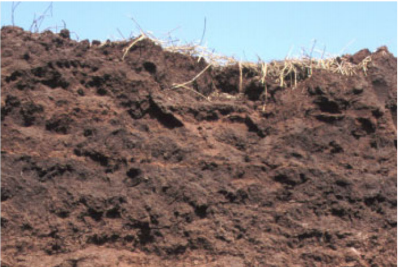
\includegraphics[width=0.8\textwidth]{soil_profile.png}
	\caption{某地土壤切面图,来源 https://www.nrcs.usda.gov}
	\label{soil_profile}
\end{figure}

1. 简单几何模型不能模拟土壤表面复杂的起伏特征。如图\ref{soil_profile}所示,真实土壤表面呈现凹凸不平的起伏特征,这将会在雷达回波中
引入相当程度的抖动等干扰,而常规仿真方法中使用的标准长方体模型的边界是完美的平面,不能代表实际土壤的形态。所以需要研究土壤表面起伏
的数据特征并构想相关的模型生成算法。

2. 均匀介质模型不能模拟土壤中介质的随机分布特征。观察图\ref{soil_profile}中的土壤剖面可看到不均匀的土壤颗粒分布特征,土壤中介质
的不均匀分布必将导致雷达波传播过程中的路径和散射特征的改变,从来对雷达B扫图像引起干扰。常规方法中所使用的均匀介质,除了在不同介质的
相交面这样的介质参数突变的位置,对雷达波不会产生任何扭曲和路径改变,产生的数据过于理想化。因此需要研究土壤介质的构成模型和分布特点
并提供相应的建模算法以模拟真实土壤的介质形态。

3. 点源模型不能模拟近场状态时天线的传输特征。常规仿真方法通常将探地雷达天线近似为单个网格的点源模型,但是由于本文所研究的目标识别问题
中目标和天线的距离较近,且该距离接近天线的工作频率波长,因此此时天线的传输特征对雷达B扫图像将产生可见的影响,不符合尽量获取拟真数据
的目标,因此继续使用常规方法中的点源模型将不是理想的选择。

本章主要内容安排为:1. 介绍FDTD仿真的基本原理和开源数值仿真平台Gprmax;2. 针对模拟土壤表面复杂起伏特征和介质随机
分布特征的问题,基于土壤介质参数半经验模型和FFT分形数据生成算法形成真实土壤模型构建算法;3. 针对模拟天线传输特征的问题,
研究将真实天线几何模型内置到FDTD网格的方法。4. 综合前面几节的结果,批量得到拟真雷达B扫图像。
\section{仿真方法与计算平台}
常用的电磁仿真方法有矩量法、有限元法和FDTD法。其中有限元法的理论基础是变分和插值,适用于求解各类微分方程问题,特别是物理场的求解问题;
矩量法的求解目标是代数方程组,这些方程组由待求解积分或微分方程转化而来;FDTD法以差分原理为基础,将麦克斯韦方程中的微分算子通过差分近似。
FDTD法具有容易掌握,直观简洁的特点,其计算迭代方程可由麦克斯韦方程直接导出而且不需要进行其他复杂的推导过程,另外由于其将空间划分为均匀的
立方体网格,所以也特别适合复杂模型的程序化生成,特别是本章要解决的土壤与天线建模问题。
\subsection{FDTD方法基本原理}
\begin{figure}[htbp]
	\includegraphics{yee_cube.pdf}
	\caption{FDTD网格示意图}
	\label{yee_cube}
\end{figure}

FDTD法的基本思想是将计算空间离散为一个一个的矩形网格(图\ref{yee_cube}),然后再将磁场与电场矢量分布到这些网格上,其中磁场位于每个立方体各个面的重心处且
垂直于该表面,电常位于各条边中心且与其平行。将$\mathbf{E}_x$、$\mathbf{E}_y$、$\mathbf{E}_z$、
$\mathbf{H}_x$、$\mathbf{H}_y$、$\mathbf{H}_z$六个分量以Maxwell方程组联系起来,即可得到:
\begin{equation} 
\varepsilon \frac{\partial E_{x}}{\partial t}=\frac{\partial H_{z}}{\partial y}-\frac{\partial H_{y}}{\partial z}-\sigma E_{x}
\label{eqn:maxwell_1} 
\end{equation}
 \begin{equation} 
 \varepsilon \frac{\partial E_{y}}{\partial t}=\frac{\partial H_{x}}{\partial z}-\frac{\partial H_{z}}{\partial x}-\sigma E_{y}
  \end{equation}
  \begin{equation} 
  \varepsilon \frac{\partial E_{z}}{\partial t}=\frac{\partial H_{y}}{\partial x}-\frac{\partial H_{x}}{\partial y}-\sigma E_{z}
   \end{equation}
   \begin{equation} 
\mu \frac{\partial H_{x}}{\partial t}=\frac{\partial E_{y}}{\partial z}-\frac{\partial E_{z}}{\partial y}
 \end{equation}
 \begin{equation} 
\mu \frac{\partial H_{y}}{\partial t}=\frac{\partial E_{z}}{\partial x}-\frac{\partial E_{x}}{\partial z}
 \end{equation}
 \begin{equation} 
	\label{eqn:maxwell_6}
\mu \frac{\partial H_{z}}{\partial t}=\frac{\partial E_{x}}{\partial y}-\frac{\partial E_{y}}{\partial x}
 \end{equation}

 以上6个分量均可由对于三个空间方向以及时间方向的偏导数,也就是对于$x, y, z, t$的偏导数都可以以下中心差分公式
 近似表示:
 \begin{equation} 
 \frac{\partial f(\xi)}{\partial \xi}=\frac{\partial f(\xi+\Delta \xi / 2)}{\partial \xi}-\frac{\partial f(\xi-\Delta \xi / 2)}{\partial \xi}
  \end{equation}

代入式\ref{eqn:maxwell_1}-\ref{eqn:maxwell_6}即可得到Maxwell方程的离散形式:
\begin{equation} 
\begin{array}{l}{E_{x}^{n+1}\left(i+\frac{1}{2}, j, k\right)=\left(\frac{2 \varepsilon-\sigma \Delta t}{2 \varepsilon+\sigma \Delta t}\right) E_{x}^{n}\left(i+\frac{1}{2}, j, k\right)+\left(\frac{2 \Delta t}{2 \varepsilon+\sigma \Delta t}\right)\{ } \\ {\frac{1}{\Delta y}\left[H_{z}^{n+\frac{1}{2}}\left(i+\frac{1}{2}, j+\frac{1}{2}, k\right)-H_{z}^{n+\frac{1}{2}}\left(i+\frac{1}{2}, j-\frac{1}{2}, k\right)\right]-} \\ {\frac{1}{\Delta z}\left[H_{y}^{n+\frac{1}{2}}\left(i+\frac{1}{2}, j, k+\frac{1}{2}\right)-H_{y}^{n+\frac{1}{2}}\left(i+\frac{1}{2}, j, k-\frac{1}{2}\right)\right]}\end{array}
 \end{equation}
 \begin{equation} 
\begin{array}{l}{E_{y}^{n+1}\left(i, j+\frac{1}{2}, k\right)=\left(\frac{2 \varepsilon-\sigma \Delta t}{2 \varepsilon+\sigma \Delta t}\right) E_{y}^{n}\left(i, j+\frac{1}{2}, k\right)+\left(\frac{2 \Delta t}{2 \varepsilon+\sigma \Delta t}\right)\{ } \\ {\frac{1}{\Delta z}\left[H_{x}^{n+\frac{1}{2}}\left(i, j+\frac{1}{2}, k+\frac{1}{2}\right)-H_{x}^{n+\frac{1}{2}}\left(i+\frac{1}{2}, j, k-\frac{1}{2}\right)\right]-} \\ {\frac{1}{\Delta x}\left[H_{z}^{n+\frac{1}{2}}\left(i+\frac{1}{2}, j+\frac{1}{2}, k\right)-H_{z}^{n+\frac{1}{2}}\left(i-\frac{1}{2}, j+\frac{1}{2}, k\right)\right]}\end{array}
 \end{equation}
 \begin{equation} 
\begin{array}{l}{E_{z}^{n+1}\left(i, j, k+\frac{1}{2}\right)=\left(\frac{2 \varepsilon-\sigma \Delta t}{2 \varepsilon+\sigma \Delta t}\right) E_{z}^{n}\left(i, j+\frac{1}{2}, k\right)+\left(\frac{2 \Delta t}{2 \varepsilon+\sigma \Delta t}\right)\{ } \\ {\frac{1}{\Delta x}\left[H_{y}^{n+\frac{1}{2}}\left(i+\frac{1}{2}, j, k+\frac{1}{2}\right)-H_{y}^{n+\frac{1}{2}}\left(i-\frac{1}{2}, j, k+\frac{1}{2}\right)\right]-} \\ {\frac{1}{\Delta y}\left[H_{x}^{n+\frac{1}{2}}\left(i, j+\frac{1}{2}, k+\frac{1}{2}\right)-H_{x}^{n+\frac{1}{2}}\left(i, j-\frac{1}{2}, k+\frac{1}{2}\right)\right]}\end{array}
 \end{equation}
 \begin{equation} 
\begin{array}{l}{H_{x}^{n+\frac{1}{2}}\left(i, j+\frac{1}{2}, k+\frac{1}{2}\right)=\left(\frac{2 \mu-\sigma \Delta t}{2 \mu+\sigma \Delta t}\right) H_{x}^{n-\frac{1}{2}}\left(i, j+\frac{1}{2}, k+\frac{1}{2}\right)-} \\ {\left(\frac{2 \Delta t}{2 \mu+\sigma \Delta t}\right)\left\{\frac{1}{\Delta y}\left[E_{z}^{n}\left(i, j+1, k+\frac{1}{2}\right)-E_{z}^{n}\left(i, j, k+\frac{1}{2}\right)\right]-\right.} \\ {\frac{1}{\Delta z}\left[E_{y}^{n}\left(i, j+\frac{1}{2}, k+1\right)-E_{y}^{n}\left(i, j+\frac{1}{2}, k\right)\right]}\end{array}
 \end{equation}
 \begin{equation} 
\begin{array}{l}{H_{y}^{n+\frac{1}{2}}\left(i+\frac{1}{2}, j, k+\frac{1}{2}\right)=\left(\frac{2 \mu-\sigma \Delta t}{2 \mu+\sigma \Delta t}\right) H_{y}^{n-\frac{1}{2}}\left(i+\frac{1}{2}, j, k+\frac{1}{2}\right)-} \\ {\left(\frac{2 \Delta t}{2 \mu+\sigma \Delta t}\right)\left\{\frac{1}{\Delta z}\left[E_{x}^{n}\left(i+\frac{1}{2}, j, k+1\right)-E_{z}^{n}\left(i+\frac{1}{2}, j, k\right)\right]-\right.} \\ {\frac{1}{\Delta x}\left[E_{z}^{n}\left(i+1, j, k+\frac{1}{2}\right)-E_{z}^{n}\left(i, j, k+\frac{1}{2}\right)\right]}\end{array}
 \end{equation}
 \begin{equation} 
\begin{array}{l}{H_{z}^{n+\frac{1}{2}}\left(i+\frac{1}{2}, j+\frac{1}{2}, k\right)=\left(\frac{2 \mu-\sigma \Delta t}{2 \mu+\sigma \Delta t}\right) H_{z}^{n-\frac{1}{2}}\left(i+\frac{1}{2}, j+\frac{1}{2}, k\right)-} \\ {\left(\frac{2 \Delta t}{2 \mu+\sigma \Delta t}\right)\left\{\frac{1}{\Delta x}\left[E_{y}^{n}\left(i+1, j+\frac{1}{2}, k\right)-E_{z}^{n}\left(i, j+\frac{1}{2}, k\right)\right]-\right.} \\ {\frac{1}{\Delta y}\left[E_{x}^{n}\left(i+\frac{1}{2}, j+1, k\right)-E_{x}^{n}\left(i+\frac{1}{2}, j, k\right)\right]}\end{array}
 \end{equation}

通过以上各式,在$t_0$时刻已知当前空间所有网格电场值的情况下,便可推得$t_0+{\Delta t}/2$时刻所有网格的磁场值,
再次步进${\Delta t}/2$时刻即又能得到$t_0+\Delta t$时刻的电场值。如此循环往复即可进行电磁波在自由空间与介质中
随时间传播的数值模拟结果。以上是FDTD方法的时间步进基本过程,关于其数值稳定性、误差分析和边界条件等细节在此便不再赘述。
\subsection{Gprmax仿真平台}
通过上节的原理很容易自行编写可用的FDTD数值计算程序。笔者曾编写过基于C++与Matlab的三维FDTD仿真软件,两种程序均存在
一些难以克服的缺点。Matlab版由于Matlab强大的工程计算函数库和友好的界面很容易进行快速建模与结果可视化,但是其计算缓慢
,即使使用内置的并行接口其速度也难以达到本文的计算量需求。C语言版可生成高效原生代码,并且可借助并行计算程序包OpenMP在
实验室数值计算服务器上利用多核CPU的优势得到更快的计算速度。但是相对于Matlab版,C语言版却缺乏足够的灵活性,在复杂形体建模
方面需要书写大量的底层逻辑甚至需要用到专业的计算几何知识,此外C语言在数据的可视化方面也缺乏足够的工具,往往还是需要
借助其他工具进行数据处理。考虑到这些因素,本文采用英国爱丁堡大学团队开发的开源电磁仿真程序包Gprmax作为FDTD计算引擎,并
利用其开源的优势进行大量的二次开发以满足本文中建模仿真的需要。

结合本文所研究问题的实际特点,Gprmax 与C、Matlab以及其他常见商业软件相比以下显著优势:

计算速度快。最新版Gprmax采用python语言开发,python作为一门脚本语言本身运行效率并不高,但是却可因为其胶水语言的特性
克服这一缺点。其主要加速途径主要有三方面:1. 可以对Gprmax源码进行研究可发现内部其使用了Cython程序包。
Cython程序包可将普通的Python语句编译到C语言,从而解决解释性语言运行速度慢的问题。2. FDTD时间步进方程在计算时每个网格
场值只与上一时刻的场值有关,每个网格的计算是互相独立,因此可将计算空间划分为多个区域,并将每个区域分配给单独的CPU核心计算。
另外,在同时仿真多个模型时,还可以利用MPI调度集群内的多个CPU同时计算并汇总计算结果。3. 最新版本的Gprmax开始支持基于英伟达
CUDA平台的GPU加速,实测利用显卡的多核心矩阵运算能力可将计算时间缩短到之前的四十分之一左右。

极强的可扩展性。Gprmax 的扩展能力使得用户可以很方便的定义属于自己的模型库和脚本化控制仿真的运行,特别适合需要建立复杂模型
与大量仿真的情形。在阅读其源码后也可以对内部计算流程进行修改和补充,比如改变仿真结果的保存格式。Gprmax的扩展能力一方面来自于
其开源的特点,即所有代码可供用户阅读与修改,另一方面由于python语言在运行时不需要编译,用户所作的修改和自定义库可以和原有Gprmax
程序无缝融合而不需要传统软件工程的构建流程,方便了使用者的自定义流程。

本章后面小节的建模与仿真充分利用了这两个优势。首先土壤天线建模和补充均以python用户模块的形式增强Gprmax原有的功能。其次
仿真时均利用实验室高性能显卡实现了显著加速。

\section{拟真土壤模型}
本节所介绍的拟真土壤模型由两方面的理论组成,其一是土壤混合物的电磁参数模型,其二是地下介质分布和地形所蕴含的分形特征。
\subsection{拟真土壤模型原理}
Peplinski 等人提出一种模拟真实土壤电磁特性的半经验模型。在此模型中,土壤由三种成分构成,分别是:
颗粒直径在0.05mm到2.0mm之间的沙土,颗粒直径在0.002mm到0.05mm之间的粉土,以及颗粒直径在0.002
以下的粘土。这三种成分的配比不同可表示不同的土壤类型,进而也影响到其电磁特性。同时,土壤中含水量也对
其电磁特性起重大影响。综合这些因素,土壤的复介电常数$\epsilon_m$由式\ref{eqn:peplinskiall}给出。
\begin{equation} 
	\label{eqn:peplinskiall} 
	\begin{aligned} \epsilon_{m} &=\epsilon_{m}^{\prime}-j \epsilon_{m}^{\prime \prime} \\ 
\epsilon_{m}^{\prime} &=1.15 \left[1+\frac{\rho_{b}}{\rho_{s}}\left(\epsilon_{s}^{\alpha}\right)+m_{v}^{\beta^{\prime}} \epsilon_{f w}^{\alpha}-m_{v}\right]^{1 / \alpha} - 0.68\\ 
\epsilon_{m}^{\prime \prime} &=\left[m_{v}^{\beta^{\prime \prime}} \epsilon_{f w}^{\prime \prime \alpha}\right]^{1 / \alpha} \end{aligned}
\end{equation}

上式中,$\epsilon_{m}^{\prime}$ 与 $\epsilon_{m}^{\prime}$分别是复介电常数
$\epsilon_m$的实部与虚部;$\rho_{b}$ 与 $\rho_{s}$分别是土壤的总密度和其中沙土成分
的密度(单位:$g/cm^3$);$\beta^\prime$与$\beta^{\prime \prime}$分别是与土壤构成
相关的常数,其表达式为\ref{eqn:soil_beta},其中$S$与$C$分别是沙土与粘土的构成比例
($0<S<1, 0<C<1$)。
\begin{equation} 
	\label{eqn:soil_beta}
	\begin{aligned}
\beta^{\prime}&=1.2748-0.519 S-0.152 C \\
\beta^{\prime \prime}&=1.33797-0.603 S-0.166 C
	\end{aligned}
\end{equation}

式\ref{eqn:peplinskiall}中$\epsilon_{f w}^{\prime}$与$\epsilon_{f w}^{\prime \prime}$
分别是土壤中自由水的实部与虚部,其表达式由式\ref{eqn:soil_water}给出。
\begin{equation} 
	\label{eqn:soil_water}
	\begin{aligned}
		\epsilon_{f w}^{\prime}&=\epsilon_{w \infty}+\frac{\epsilon_{w 0}-\epsilon_{w \infty}}{1+\left(2 \pi f \tau_{w}\right)^{2}} \\
		\epsilon_{f w}^{\prime \prime}&=\frac{2 \pi f \tau_{w}\left(\epsilon_{w 0}-\epsilon_{w \infty}\right)}{1+\left(2 \pi f \tau_{w}\right)^{2}}+\frac{\sigma_{\mathrm{eff}}}{2 \pi \epsilon_{0} f} \frac{\left(\rho_{s}-\rho_{b}\right)}{\rho_{s} m_{v}}
	\end{aligned}
\end{equation}
其中,$\epsilon_{w \infty}$是$\epsilon_{f w}^{\prime}$在高频时的极限;$\tau_{w}$为自由水的
弛豫时间常数;$\epsilon_{w 0}$为水的静态相对介电常数,其值为80.1;$\sigma_{\mathrm{eff}}$为有效电导率
,由经验公式\ref{eqn:soil_eff}给出。
\begin{equation}
	\label{eqn:soil_eff}
\sigma_{\mathrm{eff}}=0.0467+0.2204 \rho_{b}-0.4111 S+0.6614 C
\end{equation}

以上便是拟真土壤模型的基本原理,下面讨论如何将此模型应用到探地雷达FDTD仿真中。
按照式\ref{eqn:peplinskiall},在给定土壤构成比例$S$与$C$后,该土壤类型的电磁参量主要由含水量决定。
实际土壤中含水量的分布不是均匀的,因此可定义含水量的最小值与最大值分别为$m_{vmin}$与$m_{vmax}$。
将此含水量范围等距离取$n$个点并代入式\ref{eqn:peplinskiall}便可得到一系列复介电常数
$\epsilon_i(i=1,2,3...n)$ 

得到组成土壤的介质列表之后,接下来了的问题便是考虑这些介质应该如何分布在FDTD三维网格中。文献(https://www.cambridge.org/core/books/fractals-and-chaos-in-geology-and-geophysics/FA8339855DBBF054CCF18D8E5DDFFAC9)
指出地下空间内孔隙度含水量等特性的分布并不是完全随机的而是呈随机分形特征。因此可以利用分形生成算法安排前面得到的一系列介质在FDTD网格
中的分布从而达到对真实土壤较好的模拟效果。

分形在数学中是一种抽象的物体,用于描述自然界中存在的事物。人工分形通常在放大后能展现出相似的形状。 
分形也被称为扩展对称或展开对称。如果在每次放大后,
形状的重复是完全相同的,这被称为自相似。分形在不同的缩放级别上可以是近似相似的。 
分形也包有图像的细节重复自身的意味。一种效率较高的分形数据生成算法是以离散傅里叶变换为基础的。
其算法理论基础是具有分形特征的数据的离散傅里叶变换(DFT)上各频率
的系数$m_f$与频率$f$近似呈幂律关系,即:
\begin{equation}
m_f = \frac{C}{f^{\frac{-(2 D-7)}{2}}}
\end{equation}
其中$D$为分形维度,其值在1到3之间。

因此,可以用以下步骤生成生成复介电常数列表在土壤所在三维空间内FDTD网格的分形分布:

1. 对于尺寸为$x,y,z$的FDTD网格区域,生成相同大小的随机三维数据$\mathbf{A}$。

2. 对$\mathbf{A}$应用三维快速傅里叶变换算法,并将结果进行平移,使零频率处于三维数组
的中心。

3. 设$\mathbf{A}$的中心点的坐标为$(i_c,j_c,k_c)$,对于每一个数据点$\mathbf{A}(i,j,k)$
,计算其与中心点的模,即$L=\sqrt{(i - i_c)^2 + (j - j_c)^2 + (k - j_c)^2}$。

4. 应用公式 $\mathbf{A}(i,j,k) = \mathbf{A}(i,j,k) \frac{1}{L^{\frac{-(2 D-7)}{2}}}$。

5. 对$\mathbf{A}$进行逆傅里叶变换,并将结果归一化并量化为$1$到$n$的整数(对应土壤介质的个数),并在对应位置为FDTD网格的赋予相应
的介质参数。

要获得高度拟真的土壤模型,除了要考虑介质参数分布方面的特征,还要考虑到地形的特征。和土壤介质的分布一样,土壤表面起伏的
形态也符合分形的特征(图\ref{soil_profile})。

由于同样满足分形特征,土壤起伏表面也可由上述类似的方式生成,比较重要的变化是上面三维的数据变为二维的数据,
空间上的三维傅里叶变换变成平面上的二维傅里叶变换,但是其算法本质不变。其过程可描述为(定义土壤起伏程度为
$k$,分形维数为$D$:

1. 对于尺寸为$x,y$的FDTD网格区域(该区域为需要生成土壤起伏表面的土壤区域顶部所围成的二维区域),
生成相同大小的随机二维数据$\mathbf{A}$。

2. 对$\mathbf{A}$应用二维快速傅里叶变换算法,并将结果进行平移,使零频率处于二维数组
的中心。

3. 设$\mathbf{A}$的中心点的坐标为$(i_c,j_c)$,对于每一个数据点$\mathbf{A}(i,j)$
,计算其与中心点的模,即$L=\sqrt{(i - i_c)^2 + (j - j_c)^2}$。

4. 应用公式 
\begin{equation}
	\label{eqn:fractal_2d}
	\mathbf{A}(i,j) = \mathbf{A}(i,j) \frac{1}{L^{\frac{-(2 D-7)}{2}}}
\end{equation}

5. 对$\mathbf{A}$进行逆傅里叶变换,将所得结果归一化到$[-k,k]$范围内,此时$\mathbf{A}$即代表
土壤区域顶部对应的起伏程度,将此起伏程度数据应用于建模过程便可得到具有起伏表面的土壤模型。
\subsection{建模实例}
为了方便展示计算过程,这里对土壤起伏表面的生成过程做建模演示。图\ref{rough_surface}展示了上述土壤分形生成算法
中各步骤的计算结果,其中第一步中$x$和$y$的值皆为400,分形维数$D=1.5$。图\ref{rough_surface}(a)为原始随机矩阵,
在经过傅里叶变换后变为图\ref{rough_surface}(b),频域数据经过公式\ref{eqn:fractal_2d}处理后能量集中到
低频区域,这一点可在图\ref{rough_surface}(c)看出来,其中能量由图中心的低频部分像周围的高频区域逐渐下降(图中的
颜色以对数尺度标出)。最后,如图\ref{rough_surface}{d}所示,恢复到时域的数据呈现类似于地形起伏的分形特征。
\begin{figure}[htbp]
	\subfigure[]{
		\label{rough_surface_a}
		\includegraphics{rough_surface_random.pdf}}
	\subfigure[]{
		\label{rough_surface_b}
		\includegraphics{rough_surface_fft.pdf}}
	\subfigure[]{
		\label{rough_surface_c}
		\includegraphics{rough_surface_fft_fractal.pdf}}
	\subfigure[]{
		\label{rough_surface_d}
		\includegraphics{rough_surface_fractal.pdf}
	}
	\caption{土壤起伏表面建模实例二维图。(a)随机二维数据;(b)随机数据的二维傅里叶变换;
	(c)应用公式\ref{eqn:fractal_2d}后的结果;(d)最后生成的土壤起伏数据}
	\label{rough_surface}
\end{figure}

直观起见,图\ref{rough_surface_3d}给出了\ref{rough_surface}(d)中数据的三维曲面图。设该曲面所代表的数据为
$\mathbf{A}_{fractal}$,且其最大值为$A_{max}$最小值为$A_{min}$。在将该结果应用到FDTD建模之前需要对其值的范围进行调整,若指定模型中该土壤表面高度值的
范围为$h_{min}$到$h_{max}$,则可根据下面的公式得出在FDTD模型中的实际表面高度。
\begin{equation}
	\mathbf{A}_{fractal} = \mathbf{A}_{fractal} \frac{h_{max} - h_{min}}{A_{max} - A_{min}} + 
		h_{min} - (\frac{h_{max} - h_{min}}{A_{max} - A_{min}}) h_{min}
\end{equation}
\begin{figure}[htbp]
	\includegraphics[]{rough_surface_fractal_3d.pdf}
	\caption[]{土壤起伏表面建模实例三维图}
	\label{rough_surface_3d}
\end{figure}

按照前述类似的过程也可以建立前述土壤介质分布模型,将此模型与起伏表面模型结合起来便得到完整的拟真土壤模型(图\ref{soil_model_3d})。


\begin{figure}[htbp]
	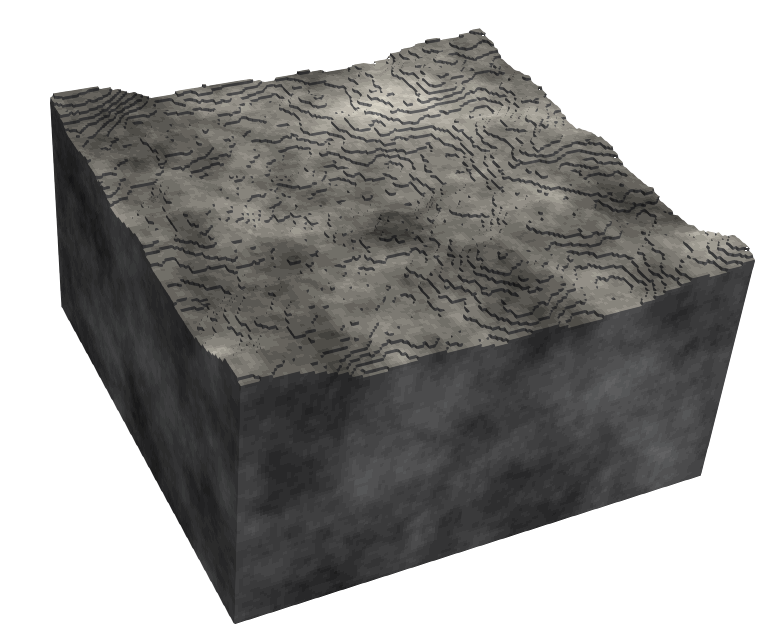
\includegraphics[width=0.8\textwidth]{soil_model_3d.png}
	\caption{拟真土壤模型建模示例}
	\label{soil_model_3d}
\end{figure}
\section{天线模型仿真}
\subsection{FDTD天线模型原理}
\subsection{仿真实例}
\section{B 扫数据的批量生成}
\section{本章小结}
本章首先研究了时域积分方程时间步进算法的阻抗元素精确计算技术,分别采用DUFFY变换法与卷积积分精度计算法计算时域阻抗元素,通过算例验证了计算方法的高精度。

